\documentclass[12pt,a4paper]{article}
\usepackage[utf8x]{inputenc}
\usepackage{amssymb}
\usepackage[russian]{babel}
\usepackage[onehalfspacing]{setspace}
\usepackage{hyperref}

\usepackage{amsthm}
\usepackage{graphicx}
\usepackage{amsmath}

% Цвета в тексте 
\usepackage{xcolor}

\title{Моделирование изображений WISE профилем Серсика при помощи программ SExtractor и Tractor}
\author{Панасюк Андрей}


\begin{document}
	
\maketitle
\thispagestyle{empty}

\newpage
\tableofcontents

\newpage
\section{Обзор литературы.}

В данном разделе я кратко опишу, некоторые найденные мною статьи по теме Tractora и его применения к исследованию данных WISE.

Статья \hyperref[1]{1} говорит о проекте DESI Legacy Imaging Surveys. Их команда проводит фотометрию внегалактических источников в диапазонах grz и в полосах W1-4 исследований WISE для большого участка неба~$\approx 14,000 deg^2$.

Кадры WISE обладают не очень хорошим разрешением, поэтому авторы для измерение объектов в этой области спектра используют методику ''force photometry'', беря положения источников и их типы (звезда/галактика) из наблюдений в других диапазонах. Примером может служить статья~\hyperref[2]{2}, где описана процедура использования Tractora для фотометрии 400 миллионов SDSS источников по данным WISE. 

Также Tractor применяется для создания каталога unWISE. В статье~\hyperref[3]{3} описаны результаты последнего обновления данного ресурса, на основе сопоставления наблюдений 8 летнего периода работы WISE.

В статье, посвященной DESI говорится о том, что для создания PSF изображений, они используют программу PSFEx, которую E. Bertin разработал для SExtractora. Далее они преобразуют её используя методику, описанную в статье \hyperref[4]{4}. Саму методику я изучить не успел.

Тексты всех статей прикреплены архивом к письму.

\section{Изображения}

Для данной работы я брал изображения из обзора \href{https://irsa.ipac.caltech.edu/applications/wise/}{WISE}. В этой работе я использовал данные в фильтре $W1$ ($\lambda = 3.368 \mu m$ ), поскольку изображения в этом фильтре имеют наилучшее разрешение. В идеале, конечно, стоит использовать данные со всех четырех фильтров. 

Для освоения программ (SExtractor, Tractor) и сравнения качества их работы мне требовались модельные изображения. 
На \hyperref[pic1]{Рис. 1} представлены четыре изображения из разных областей неба. По ним я оценил среднее значение фона неба и его отклонение (\hyperref[tab1]{Таблица 1.}). 


\begin{figure}
    \begin{minipage}{0.45\linewidth}
        \center{Gal: 30:00:00 +30:00:00 \includegraphics[width=\textwidth]{/home/andrej/Desktop/kurs/workdir/Images/Gal30+30/ICORE_0001_W1_mosaic-int.jpg}
}
    \end{minipage}    
    \hfill
    \begin{minipage}{0.45\linewidth}
        \center{Gal: 30:00:00 -30:00:00
\includegraphics[width=\textwidth]{/home/andrej/Desktop/kurs/workdir/Images/Gal30-30/ICORE_0001_W1_mosaic-int.jpg}
}
    \end{minipage}
    \vfill \label{pic1}
    \begin{minipage}{0.45\linewidth}
        \center{\includegraphics[width=\textwidth]{/home/andrej/Desktop/kurs/workdir/Images/Gal130+60/ICORE_0001_W1_mosaic-int.jpg}
Gal: 130:00:00 +60:00:00}
    \end{minipage}
    \hfill
    \begin{minipage}{0.45\linewidth}
        \center{\includegraphics[width=\textwidth]{/home/andrej/Desktop/kurs/workdir/Images/Gal130-60/ICORE_0001_W1_mosaic-int.jpg}
Gal: 130:00:00 -60:00:00}
    \end{minipage}
    \caption{Пробные изображения из каталога WISE.} 
\end{figure}

\begin{table}[h]
\begin{center}
			\begin{tabular}{|c|c|c|c|}
				\hline 
				Frame & mean & median & std \\
				 \hline
				 1 & 1.7630754 & 1.7596036 & 0.04323549 \\
				 \hline 
				 2 & 2.6068091 & 2.5979652 & 0.06251362 \\
				 \hline
				 3 & 2.3416495 & 2.3137467 & 0.19154684 \\
				 \hline
				 4 & 2.5465596 & 2.5438370 & 0.03818423 \\
				 \hline
				 \textbf{MEAN} &  \textbf{2.3145234} &\textbf{2.303788125} & \textbf{0.083870045}\\
				 \hline
			\end{tabular} 
        \caption{Данные фона неба для пробных изображений.} \label{tab1}
\end{center} 		
\end{table} 

Для построения изображений я использовал пакет \href{https://github.com/GalSim-developers/GalSim}{Galsim}. За точечные источники я брал гауссианы с FWHM = 1''. Галактики моделировал профилем Серсика. Параметры для галактик:
\begin{itemize}
    \item Положение центра $xc, yc$;
    \item Поток $Flux$;
    \item Эффективный радиус $R_e$;
    \item Параметры ориентации эллипса $g_1, g_2$;
    \item Индекс Серсика $n$.
\end{itemize}

На \hyperref[pic2]{Рис. 2} приведено модельное изображение, используемое для тестов.

\begin{figure}
\center{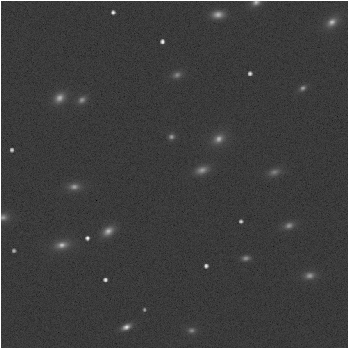
\includegraphics[width=0.5\textwidth]{model.png}
\caption{Модельное изображение. 20 галактик и 10 звезд.}} \label{pic2}
\end{figure}




\section{Tractor. Модель.}

Для освоения данной программы я использовал официальный \href{http://thetractor.readthedocs.org/en/latest/}{мануал.} К сожалению, он не полный, поэтому порой приходилось лезть в сами программные файлы, чтобы понять как работают некоторые функции.

На сколько я понял, данная программа предназначена для моделирования изображений на кадре, заданными исходными моделями методом наименьших квадратов. Таким образом необходимо предварительно обработать исходные изображения, прежде чем давать их на вход Трактору. Для модельных изображений я использовал следующий алгоритм:

\begin{enumerate}

    \item Извлечение данных из fits изображения. (Я использовал astropy.fits, автор Трактора предпочитает \href{https://github.com/esheldon/fitsio}{fitsio});
    \item Измерение фона неба и ошибки шума (Я использовал пакет \href{https://photutils.readthedocs.io/en/stable/index.html}{photutils}):
        \begin{itemize}
            \item Первичное детектирование источников с порогом 2$\sigma$, для создания маски;
            \item Измерение фона неба с полученной маской при помощи Background2D;
        \end{itemize}
    \item Поиск источников c $treshold = background + 2.0 \cdot background\_rms$ (рекомендован на сайте photutils) и десигментация, также используя функции photutils;
    \item Составление каталога из найденных источников:    
    \item Построение PSF модели при помощи функций \href{https://photutils.readthedocs.io/en/stable/psf.html#module-photutils.psf}{photutils.psf}:
        \begin{itemize}
            \item Поиск ярких объектов при помощи функции find\_peaks();
            \item Извлечение найденных объектов extract\_stars() ;
            \item Нормировка изображений на 1;
            \item Подгонка изображений при помощи Tractora гауссианой с переменной сигмой.
        \end{itemize}
    \item Полученные раннее данные даются Трактору в качестве параметров (фон неба, PSF, положения источников и поток от них)
        \begin{itemize}
            \item Из имеющихся данных я не смог придумать метод отличить галактики от звезд, поэтому я изначально провожу подгонку из расчета, что все объекты точечные. По данным остаточного изображения, я нахожу источники, которые остались не подогнанными, заменяю их на галактики и провожу повторную подгонку. 
         \end{itemize}               

     \end{enumerate}
        
Видно, что мой алгоритм очень сырой и не надежный. Он работает только для ''хороших'' модельных изображений. Так, например, если на изображении есть тесные яркие объекты, не разделенные деблендированием, или галактики яркостью больше чем звезды, то результат работы моей программы не удовлетворителен. Также возникли некоторые проблемы с построением PSF изображения. Изначально я пробовал воспользоваться функцией EPSFBuilder из пакета photutils.psf. Полученное изображение хорошо соответствовало действительности, но, как я понял, для самого Tractora изображение PSF должно быть в определенном формате, и мне не удалось их совместить между собой. Идею подгона гауссианой я почерпнул из программ, которые лежали в установочных файлах Tractora. 

Также отмечу, что Tractor очень чувствителен к исходным параметрам. Плохое определение фона или PSF могут испортить результат.
 
На графиках (\hyperref[pic3]{3}, \hyperref[pic4]{4}, \hyperref[pic5]{5}) приведены результаты, полученные при обработке модельного изображения. 


\begin{figure}
    \begin{minipage}{0.25\linewidth}
        \center{ 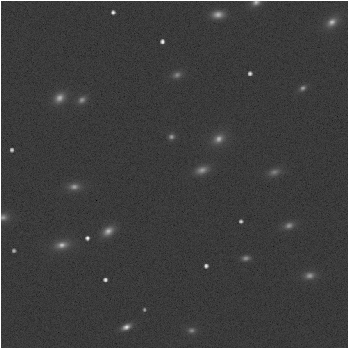
\includegraphics[width=\textwidth]{model.png} Исходное изображение.}
    \end{minipage}    
    \hfill
    \begin{minipage}{0.25\linewidth}
        \center{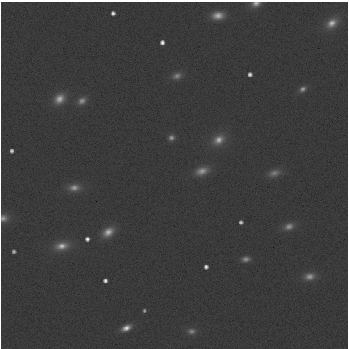
\includegraphics[width=\textwidth]{mod.png} Модель Трактора.}
    \end{minipage}
    \hfill 
    \begin{minipage}{0.25\linewidth}
        \center{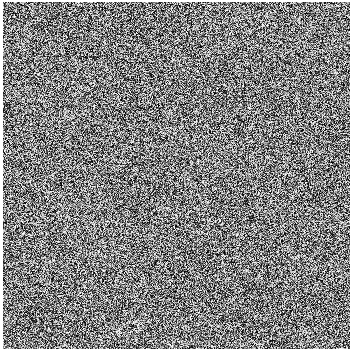
\includegraphics[width=\textwidth]{chi.png} Хи$^2$ Разность изображений.}
    \end{minipage}
    \caption{ Результат работы алгоритма Трактора} \label{pic3}
\end{figure}

\begin{figure}
    \center{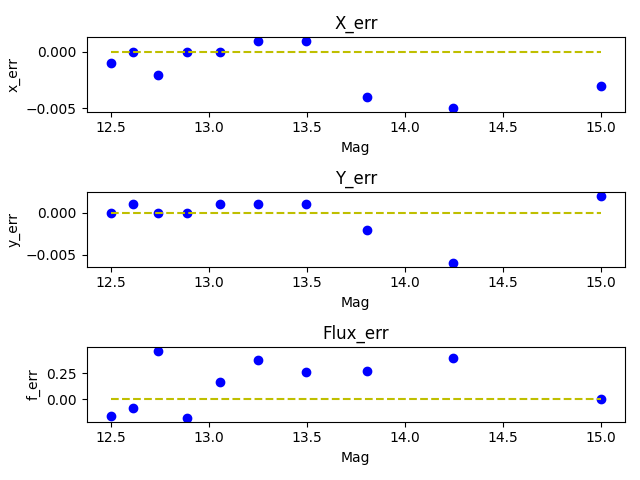
\includegraphics[width=0.6\textwidth]{p_res.png}}
    \caption{Абсолютные ошибки модельных параметров для звезд.} \label{pic4}
\end{figure}

\begin{figure}
    \center{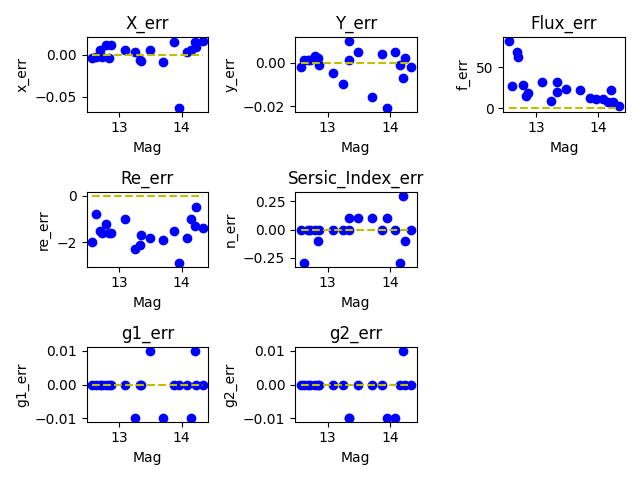
\includegraphics[width=\textwidth]{g_res.png}}
    \caption{Абсолютные ошибки модельных параметров для галактик.} \label{pic5}
\end{figure}


На данных графиках показана разность модельного значения и полученного при выполнении программы. По оси абсцисс отложено значение потока в звездных величинах. Нуль пункт шкалы 20.5 Mag. Некоторые пояснения к результатам:

\begin{itemize}
    \item В большинстве случаев положение центра объекта совпадают с модельным с хорошей точностью, как для звезд, так и для галактик;
    \item Виден недобор потока излучения от ярких галактик;
    \item Полученные ошибки для эффективного радиуса наводят меня на мысль о наличии систематических ошибок. Возможно они допущены мной при сравнении начального и итогового значений, поскольку в Тракторе все параметры задаются в пикселах, а в Galsime в угловых секундах; 
    \item Значения g1 и g2 для ориентации эллипсов хорошо подгоняются;
    \item Индекс Серсика совпадает с моделируемым для большинства объектов, независимо от их яркости.
\end{itemize}

Следует отметить, что выборка не очень показательна, поскольку рассматриваются объекты малого диапазона яркостей. Основная причина кроется в недостатках, написанного мною алгоритма. Код алгоритма доступен по \href{https://github.com/LAstroNomer/Coursework}{ссылке}.



\section{SExtractor (Source-Extractor). Модель.}

Для освоения данной программы я использовал следующие материалы: \hyperref[a]{a}, \hyperref[b]{b}, \hyperref[c]{c}. Данные инструкции не совсем полны, но в целом они дополняют друг-друга. К сожалению, в них мало примеров использования тех или иных функций.
 
Sextractor предназначен для извлечения источников из изображения и построения их каталогов. Ниже приведен список конкретных параметров, которые я извлекал из источников в данной работе:

\begin{table}[h]
    \begin{tabular}{|c|c|c|}
				\hline 
                 Параметр & Значение & Ед. Измерения\\
                \hline
                 XMODEL\_IMAGE  & X coordinate from model-fitting & [pixel] \\
                 YMODEL\_IMAGE  & Y coordinate from model-fitting & [pixel] \\
                 FLUX\_SPHEROID & Spheroid total flux from fitting  &[count]\\
                 SPHEROID\_REFF\_IMAGE & Spheroid effective radius from fitting & [pixel]\\
                 ELLIP1MODEL\_IMAGE & Ellipticity component from model-fitting & --- \\                
                 ELLIP2MODEL\_IMAGE & Ellipticity component from model-fitting & --- \\
                 SPHEROID\_SERSICNERR & RMS error on fitted spheroid Sersic index & --- \\
                 \hline
	\end{tabular} 
\end{table}


Одновременным плюсом и недостатком программы является то, что нет необходимости напрямую взаимодействовать с кодом программы. Задаются настройки работы программы и искомые параметры в файлах default.sex  и parametets.param. Также необходимо задать фильтр и $PSF$ в отдельных файлах. Также возможно использовать для фотометрии и обнаружения разные изображения, что может быть полезно, тк наши изображения в разных фильтрах имеют разное разрешение.

Как и предыдущая программа, SExtractror требует задание PSF функции в определенном формате. Для её генерации я использовал программу \href{https://github.com/astromatic/psfex}{PSFEx}. Эта программа разработана с целью создания PSF изображений для SExtractora. На \hyperref[pic6]{Рис. 6} представлено изображение PSF, полученное для модельного изображения. 

\begin{figure}[h]
    \center{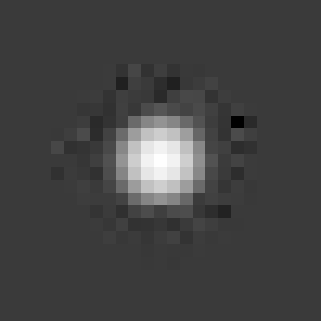
\includegraphics[width=0.5\textwidth]{PSF_Model.png}}
    \caption{PSF модель для модельного изображения} \label{pic6}
\end{figure} 

Для разделения источников на точечные и размытые у SExtractora есть параметр SPREAD\_MODEL. Как написано в \hyperref[a]{a} за критерий разделения можно взять значение $ \sqrt{ \varepsilon^2 + (k \cdot SPREADERR\_MODEL)^2 }$, где~$\varepsilon = 5 \cdot 10^{-3}$, $k = 4$. Если SPREAD\_MODEL больше этого значения, то оно считается галактикой, иначе точечным источником. Также есть объекты с отрицательным SPREAD\_MODEL, это значит, что они меньше, чем PSF функция и машина относит их к звездным потокам.
 
Ниже графиках (\hyperref[pic7]{7}, \hyperref[pic8]{8} , \hyperref[pic9]{9} ) приведены результаты работы программы. Сравнение с результатами, полученными предыдущей программой:
\begin{itemize}
        \item Не наблюдается недоучета потока для ярких источников;
        \item Немного хуже подгоняются точечные источники (черные точки на изображении Хи$^2$);
        \item Схожие между собой отклонения полученных значений эффективного радиуса, подтверждают моё предположение о систематической ошибке допущенной при сравнении результатов;
        \item Остальные параметры подгоняются примерно с той же точностью.
\end{itemize}
В результате мы можем заключить, что для полей с малой концентрацией источников программы дают приблизительно равные результаты.


\begin{figure}
    \begin{minipage}{0.25\linewidth}
        \center{ 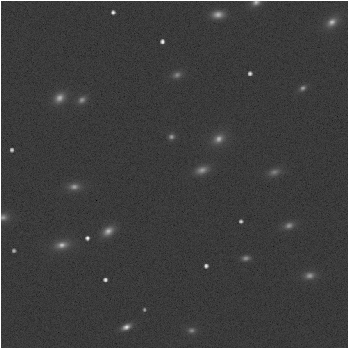
\includegraphics[width=\textwidth]{model.png} Исходное изображение.}
    \end{minipage}    
    \hfill
    \begin{minipage}{0.25\linewidth}
        \center{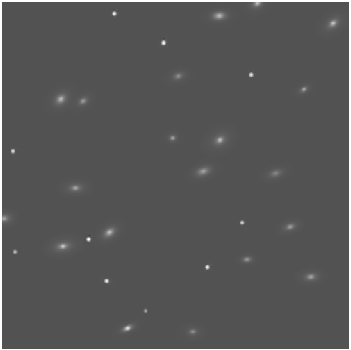
\includegraphics[width=\textwidth]{sex_mod.png} Модель Трактора.}
    \end{minipage}
    \hfill 
    \begin{minipage}{0.25\linewidth}
        \center{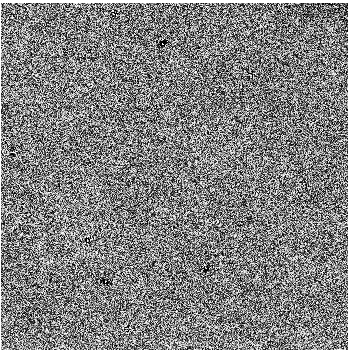
\includegraphics[width=\textwidth]{sex_sub.png} Хи$^2$ Разность.}
    \end{minipage}
    \caption{ Результат работы SExtractora} \label{pic7}
\end{figure}


\begin{figure}
    \center{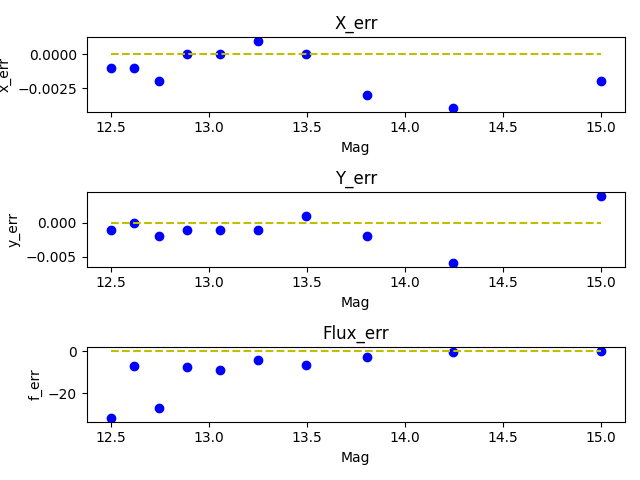
\includegraphics[width=0.6\textwidth]{se_p_res.png}}
    \caption{Абсолютные ошибки модельных параметров для звезд.} \label{pic8}
\end{figure}

\begin{figure}
    \center{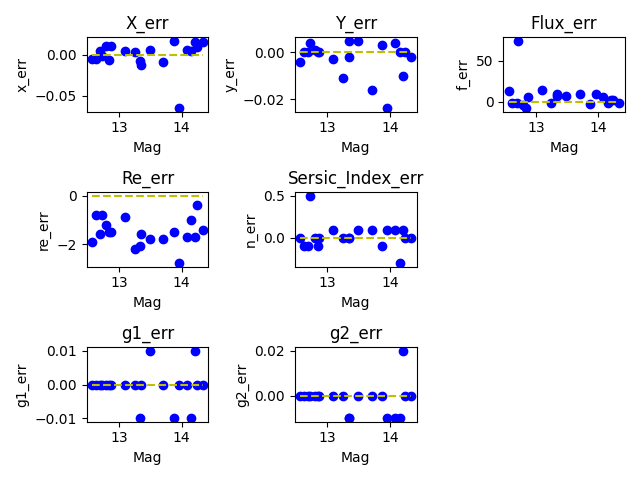
\includegraphics[width=\textwidth]{se_g_res.png}}
    \caption{Абсолютные ошибки модельных параметров для галактик.} \label{pic9}
\end{figure}


\newpage      

\section{Обработка реального изображения}

В данной части я покажу результаты работы обеих программ для кадра \hyperref[pic10a]{Рис. 10 а)} с координатами GAL +30:00:00 +30:00:00 и размером 180 угловых секунд. Согласно каталогу ALLWISE на данном кадре обнаружено 54 источника \hyperref[pic10b]{Рис. 10 б)}, но тк. часть из них находится на границе изображения их можно отбросить из объектов сравнения. Из каталога я взял значения координат источников и значение звездной величины в исследуемых фильтрах. Нуль пункт шкалы звездных величин составляет~20.5 mag для всех фильтров.

\begin{figure}[h]
    \begin{minipage}{0.45\textwidth}
        \center{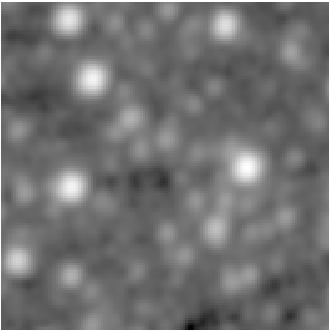
\includegraphics[width=\textwidth]{w1.png} a) Исследуемое изображение}
    \end{minipage} \label{pic10a}
    \hfill
    \begin{minipage}{0.45\textwidth}
        \center{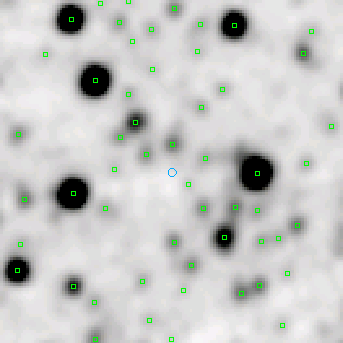
\includegraphics[width=\textwidth]{w1_cat.png} б) Объекты каталога}
    \end{minipage} \label{pic10b}
    \caption{ Кадры WISE} 
\end{figure}

Как я говорил ранее, мой алгоритм обработки изображений для Tractora не подходит для реальных кадров в связи с их плохим разрешением и большой концентрацией источников. Поэтому, я пришел к выводу, что имеет смысл источники для Tractora извлекать при помощи программы~SExtractor. PSF для обоих программ я генерировал при помощи~PSFEx. Для получения хорошей PSF функции я взял изображение той же области неба \hyperref[pic11]{Рис. 11}  размером 8x8 угловых минут.

\begin{figure}[h]
    \begin{minipage}{0.45\textwidth}
        \center{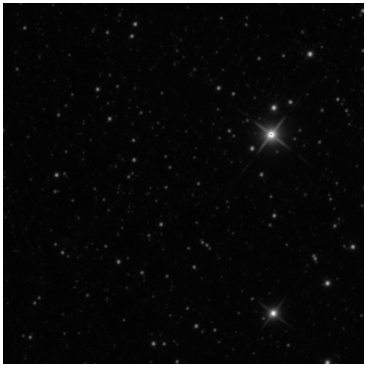
\includegraphics[width=\textwidth]{big.png} a) Большое изображение}
    \end{minipage} 
    \hfill
    \begin{minipage}{0.45\textwidth}
        \center{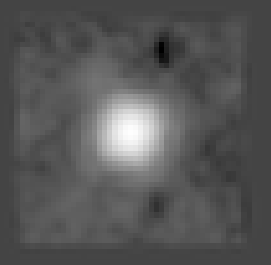
\includegraphics[width=\textwidth]{PSF.png} б) Полученная PSF}
    \end{minipage}
    \caption{ Генерация PSF модели} \label{pic11}
\end{figure}

\newpage
На \hyperref[pic12]{(Рис. 12)} представлен результат извлечения источников~SExtractor~ом. На данном кадре он нашел 58 источников (в каталоге 54), НО!:
    \begin{itemize}
        \item Часть найденных источников находятся на границе кадра и не входят в исходный каталог. Так же некоторые объекты каталога с границ кадра не были найдены вовсе. В принципе проводить фотометрию по изображениям с края кадра нехорошо, поэтому я просто не буду их брать в расчет.
        \item У некоторых объектов возникли проблемы с деблендированием. Дело в том, что в SExtractore он устроен таким образом, что не может отделить источники, если между их профилями нет провала, а на кадре присутствуют источники, для которых переход о одного к другому идет плавно, что не дает их разрешить \hyperref[pic12]{Рис. 12}. Возможно эти объекты можно различить в других фильтрах.
    \end{itemize}

\begin{figure}
    \begin{minipage}{0.45\textwidth}
        \center{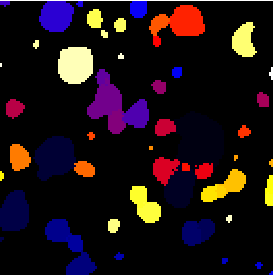
\includegraphics[width=\textwidth]{segm.png} a) Найденные изображения}
    \end{minipage} 
    \hfill
    \begin{minipage}{0.45\textwidth}
        \center{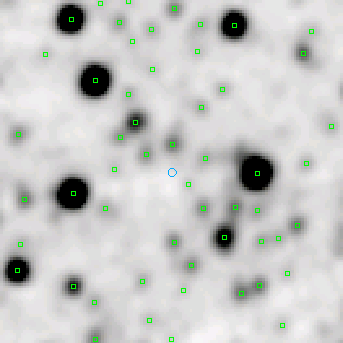
\includegraphics[width=\textwidth]{w1_cat.png} b) Изображения каталога}
    \end{minipage}
    \vfill
    \begin{minipage}{0.45\textwidth}
        \center{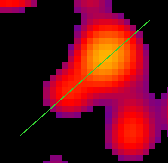
\includegraphics[width=\textwidth]{cutplot.png} c) Срез близких источников}
    \end{minipage}
    \hfill
    \begin{minipage}{0.45\textwidth}
        \center{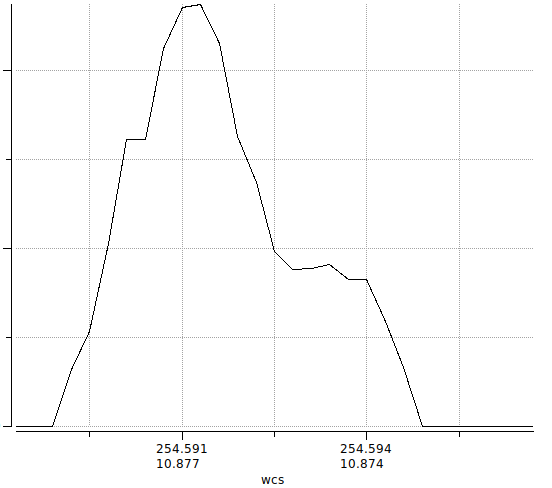
\includegraphics[width=\textwidth]{plot.png} d) Профиль яркости близких источников}
    \end{minipage}



    \caption{Поиск источников} \label{pic12}
\end{figure}

        
На \hyperref[pic13]{Рис. 13} приведены результаты моделирования SExtractora.

\begin{figure}
    \begin{minipage}{0.45\textwidth}
        \center{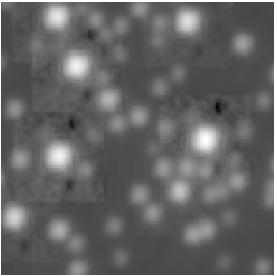
\includegraphics[width=\textwidth]{sex_p_ima.png} a) Модель точечных источников}
    \end{minipage} 
    \hfill
    \begin{minipage}{0.45\textwidth}
        \center{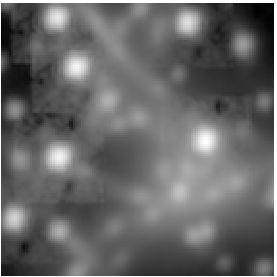
\includegraphics[width=\textwidth]{sex_g_ima.png} b) Модель галактик}
    \end{minipage}
    \vfill
    \begin{minipage}{0.45\textwidth}
        \center{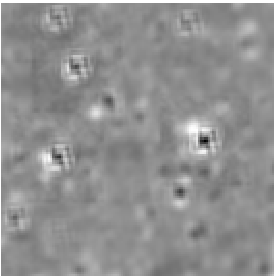
\includegraphics[width=\textwidth]{sex_p_sub.png} c) Разность точечных источников}
    \end{minipage}
    \hfill
    \begin{minipage}{0.45\textwidth}
        \center{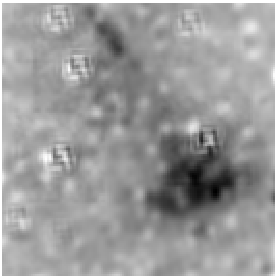
\includegraphics[width=\textwidth]{sex_g_sub.png} c) Разность галактик}
    \end{minipage}
    \caption{Результат работы SExtractora} \label{pic13}
\end{figure}

 На \hyperref[pic14]{Рис. 14} приведен результат работы Tractora. Галактики определялись по критерию описанному ранее.

Видно, что точечными источниками кадр приближается гораздо лучше, чем галактиками. Возможно это объясняется плохим качеством изображения, и, как следствие, плохим определение различия между точечными источниками и галактиками. 

\begin{figure}
    \begin{minipage}{0.45\textwidth}
        \center{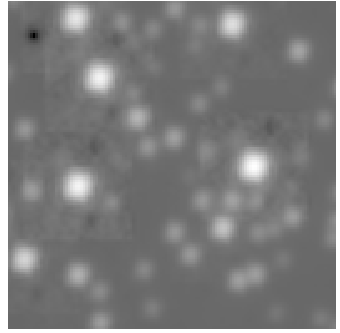
\includegraphics[width=\textwidth]{tr_p_ima.png} a) Модель точечных источников}
    \end{minipage} 
    \hfill
    \begin{minipage}{0.45\textwidth}
        \center{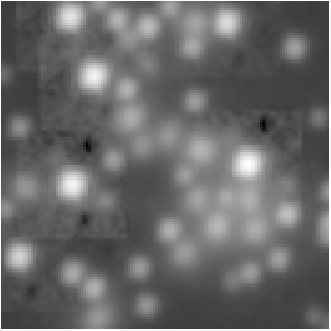
\includegraphics[width=\textwidth]{tr_g_ima.png} b) Модель галактик}
    \end{minipage}
    \vfill
    \begin{minipage}{0.45\textwidth}
        \center{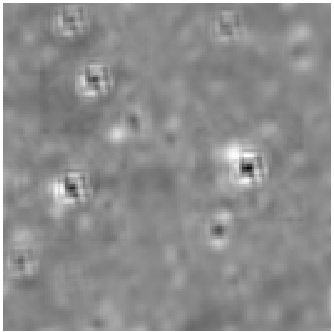
\includegraphics[width=\textwidth]{tr_p_sub.png} c) Разность точечных источников}
    \end{minipage}
    \hfill
    \begin{minipage}{0.45\textwidth}
        \center{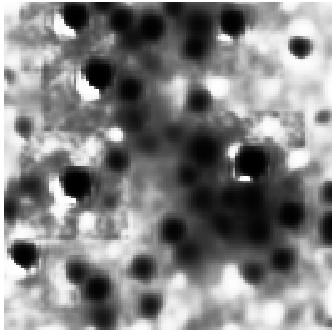
\includegraphics[width=\textwidth]{tr_g_sub.png} c) Разность галактик}
    \end{minipage}
    \caption{Результат работы Tractora} \label{pic14}
\end{figure}

\section{Обсуждение результатов}

\begin{enumerate}
    \item При применении двух программ для модельных полей было выявлено, что результаты, даваемые ими в целом сходятся. Но каждая из программ имеет некоторые недостатки, которые проявляют себя при работе с реальным изображением.
    \item Работа с реальным изображением показала, что для SExtractora недостатком является невозможность задания каким типом подгонять какие источники. Если ему задать подгонку галактиками, то в итоговом каталоге все источники будут подогнаны параметрами галактик, те необходимо проводить разделение полученных результатов. Также было выявлено, что при подгонке тесных галактик они смазываются. 
    \item Недостатком Tractora является зависимость от входных параметров, что требует определения стратегии для предварительного детектирования и разделения источников на изображении. 
    \item Возможно, что на выбранном мной снимке действительно отсутствуют галактические источники. Чтобы удостовериться в этом надо провести сравнение с другим каталогом.
\end{enumerate}

\section{Дальнейшие этапы}
     Исходя из полученных результатов можно указать следующие направления движения:
          \begin{itemize}
                \item Применение тех же алгоритмов для данных unWISE;
                \item Применение алгоритма для других фильтров (W2, W3, W4) и попробовать улучшить определение координат и морфологии на основе взаимной фотометрии и картах цвета;
                \item Придумать алгоритм связи PSF изображений каталога ALLWISE (они в формате fits) с получаемыми PSFEx и сравнить результаты; 
                \item Сравнить полученные результаты с звездными величинами для каталога ALLWISE и c данными каталога DESI.
           \end{itemize}  
  
Программы, используемые в этой работе можно найти по ссылке на github: \href{https://github.com/LAstroNomer/Coursework}{https://github.com/LAstroNomer/Coursework}    
		
\section{Список литературы}

\begin{enumerate}

\item Arjun Dey, David J. Schlegel, Dustin Lang, Robert Blum, Kaylan Burleigh, et al.. Overview of the
DESI Legacy Imaging Surveys. 2019. hal-02003991 \label{1}
\item The Astronomical Journal, 151:36 (12pp), 2016 February \label{2}
\item Aaron M. Meisner, Dustin Lang, Edward F. Schlafly, David J. Schlegel, "Eight-year Full-depth unWISE Coadds" \label{3}
\item Dustin Lang, A hybrid Fourier–Real Gaussian Mixture method for fast galaxy–PSF convolution \label{4}

\item[a] E. Bertin "SExtractor v2.13 User’s manual",Institut d’Astrophysique \& Observatoire de Paris  \label{a}
\item[b] E. Bertin "SExtractor Documentation Release 2.24.2" \label{b} 
\item[c] Benne W. Holwerda "Source Extractor for Dummies" \label{c}
\item[d] Hogg, Lang "Tractor Documentation Release 1.0" 

\end{enumerate}


\end{document}
